\documentclass[11pt]{article}


\usepackage{amsmath}
\usepackage{amssymb}
\usepackage[english, spanish,mexico]{babel}
\usepackage{amsthm}
\usepackage{bm}
\usepackage{booktabs}
\usepackage{color}
\usepackage{csquotes}
\usepackage{empheq}
\usepackage{float}
\usepackage{graphicx}
\usepackage{lipsum}
\usepackage[most]{tcolorbox}
\usepackage{mdframed}
\usepackage{multicol}
\usepackage{multirow}
\usepackage{psfrag}
\usepackage{bookmark}
\usepackage{hyperref}


\hypersetup{
   colorlinks=true,
   linkcolor=black,
   citecolor=black,
   pdftitle={Rebasando Nuevas Fronteras, la Realidad Virtual dentro de la Educación},
   urlcolor=blue
}


\usepackage{anyfontsize}
\usepackage{fontspec}
\usepackage{geometry}
\usepackage{textcase}
\usepackage{titlesec}
\usepackage{xcolor}

\usepackage[style=apa]{biblatex}

\newfontfamily{\barial}{ARIALBD}[
   Path=./fonts/ttf/,
   Extension = .ttf
]
\newfontfamily{\arial}{ARIAL}[
   Path=./fonts/ttf/,
   Extension = .ttf
]
\newfontfamily{\arialblk}{ARIBLK}[
   Path=./fonts/ttf/,
   Extension = .ttf
]
\setmainfont{calibril}[
   Path=./fonts/ttf/,
   Extension = .ttf
]
\newfontfamily{\calibri}{calibri}[
   Path = ./fonts/ttf/,
   Extension = .ttf,
   UprightFont = *-regular,
   BoldFont = *-bold,
   ItalicFont = *-italic,
   BoldItalicFont = *-bold-italic
]


\definecolor{introblock}{HTML}{DAEEF3}
\definecolor{blue}{HTML}{006999}

\newcommand\introblock[1]{\fcolorbox{introblock}{introblock}{\hspace{1em}#1\hspace{1em}}}

\titleformat{\section}
{\color{blue}\fontsize{12}{14}\arialblk}{\thesection.}{3pt}{\MakeTextUppercase}
\titleformat{\subsection}
{\color{blue}\fontsize{11}{13}\barial}{\thesubsection.}{1em}{}
\titleformat{\subsubsection}
{\color{blue}\fontsize{11}{13}\barial}{\thesubsubsection.}{1em}{}


\geometry{a4paper, left=1.18in, right=1.18in, top=0.9in, bottom=0.97in}
\linespread{1.15}
\setlength{\parindent}{0pt}



\title{\color{blue}{\fontsize{10}{12}~}\\{\arialblk\fontsize{14}{17}\selectfont Rebasando Nuevas Fronteras, la Realidad Virtual Dentro de la Educación}\\{\barial\fontsize{12}{14}\selectfont Crossing New Frontiers, Virtual Reality in Education}}

\author{
   {\arial\fontsize{12}{14}\selectfont Josué Oziel Mondragon Fernández}\\
   {\arial\fontsize{10}{12}\selectfont Universidad Autónoma de Querétaro (México)}\\
   {\arial\fontsize{10}{12}\selectfont jmondragon17@alumnos.uaq.mx}\\
   {\arial\fontsize{12}{14}\selectfont Alejandro Macias Fonseca}\\
   {\arial\fontsize{10}{12}\selectfont Universidad Autónoma Querétaro (México)}\\
   {\arial\fontsize{10}{12}\selectfont amacias15@alumnos.uaq.mx}\\
}

\date{}


\addbibresource{bibliografia-articulos-realidad-virtual.bib}

\AtBeginBibliography{\calibri}
\begin{document}
\maketitle
\begin{tcolorbox}[colback=introblock,colframe=introblock]
\section*{\fontsize{10}{12}\barial Resumen}
      {\fontsize{10}{12}La Realidad Virtual (RV) está en un punto en el cual puede llegar a revolucionar la educación, ofreciendo a los estudiantes una experiencia de aprendizaje inmersiva que trasciende los enfoques convencionales. Este artículo explorará en profundidad cómo la RV está transformando las aulas y cómo podría cambiar el futuro de la educación. Mientras la RV permite a los estudiantes adentrarse en entornos tridimensionales que simulan situaciones del mundo real o conceptos abstractos, esto mismo ofrece ventajas notables para mejorar la retención y comprensión del conocimiento adquirido. Además, la colaboración y el aprendizaje se fomentan a través de proyectos virtuales. Estos desafíos se analizan mediante el apoyo de recolección de información de otras fuentes bibliográficas adquiridas en bases de datos como Google Académico (258,000 articulos encontrados, 7 utilizados) y Elsevier (1858 articulos encontrados, 13 utilizados), considerando la calidad de los mismos. Una de las fuentes principales de información ha sido la revista \textit{Computers \& Education: X Reality}, donde se habla a fondo acerca de las tecnologías que pueden ser implementadas y ayudar en la educación, utilizando las palabras clave \textit{virtual reality, education} (también traducida respectivamente al español). Con base en el análisis hecho de las fuentes de información, la RV puede llegar a ser una gran herramienta en la educación, mas no puede reemplazar partes importantes del sistema educativo tradicional, ya que se puede llegar a adicciones o sobre estimulación donde la experiencia de aprendizaje puede llegar a ser deslindada.} 

\section*{\fontsize{10}{12}\barial Palabras Clave}
   {\fontsize{10}{12}Educacion;Nuevas tecnologías;Realidad Virtual}
\end{tcolorbox}

\begin{tcolorbox}[colback=introblock,colframe=introblock]
   \selectlanguage{english}
\section*{\fontsize{10}{12}\barial Abstract}
      {\fontsize{10}{12}Virtual Reality (VR) is at a point where it could revolutionize the education, offering students an immersive learning experience that can transcend the conventional teaching. This article will explore profoundly how VR is transforming the classrooms and how it could change the future of education. While VR allows students to immerse in 3D spaces that simulate real-world situations or abstract concepts. This offers notable improvements for information retention and acquired knowledge comprehension; also, the collaboration and learning are fomented through virtual projects. These challenges are analyzed with the support of recollected information from various sources, such as Google Scholar (258,000 articles found, 7 used) and Elsevier (1858 articles found, 13 used), considering their quality. One of the main sources of information was \textit{Computers \& Education: X Reality}, which talks profoundly about the technologies that could be implemented and help in the education sector. The keywords used were \textit{virtual reality, education}. With the analysis of the information sources, VR could be a great tool in education, but it can't replace the important qualities of the traditional educational system, because these devices can lead to addictions, or over stimulation where the learning experience could flinch.}

\section*{\fontsize{10}{12}\barial Keywords}
   {\fontsize{10}{12}Education;New Technologies;Virtual Reality}
\selectlanguage{spanish}
\end{tcolorbox}
\documentclass[11pt]{article} %5 a 8 cuartillas

\usepackage{amsmath}
\usepackage{amssymb}
\usepackage[english, spanish,mexico]{babel}
\usepackage{amsthm}
\usepackage{bm}
\usepackage{biblatex}
\usepackage{booktabs}
\usepackage{color}
\usepackage{csquotes}
\usepackage{empheq}
\usepackage{float}
\usepackage{geometry}
\usepackage{graphicx}
\usepackage{lipsum}
\usepackage{mdframed}
\usepackage{multicol}
\usepackage{multirow}
\usepackage{psfrag}
\usepackage{bookmark}
\usepackage{hyperref}
%\usepackage{fontspec}
% Adittional packages


%\renewcommand{\tiny}{\normalsize}
%\renewcommand{\footnotesize}{\normalsize}
%\renewcommand{\small}{\normalsize}
%\renewcommand{\large}{\normalsize}
%\renewcommand{\Large}{\normalsize}
%\renewcommand{\LARGE}{\normalsize}
%\renewcommand{\huge}{\normalsize}
%\renewcommand{\Huge}{\normalsize}
%\setmainfont{Arial}

\hypersetup{
   colorlinks=true,
   linkcolor=black,
   citecolor=black,
   pdftitle={Rebasando Nuevas Fronteras, la Realidad Virtual dentro de la Educación},
   urlcolor=blue
}

\geometry{a4paper, left=4cm, right=2cm, top=3cm, bottom=3cm}
\linespread{1.5}
\addbibresource{bibliografia-articulos-realidad-virtual.bib}


\title{Rebasando Nuevas Fronteras, la Realidad Virtual dentro de la Educación\\ {\large Crossing New Frontiers, Virtual Reality in Education}}
\author{Mondagrón Fernández J. O., Macías Fonseca A.}
%\course{Introducción a la Investigación}
%\professor{Sánchez Hernández Dulce Carolina}
%\duedate{Noviembre 28, 2023}
%\shorttitle{Realidad Virtual dentro de la Educación}
\date{\today} % deadline: 2023-11-28
\begin{document}
\maketitle

%\tableofcontents
%\listoffigures
%\listoftables

   \begin{abstract}
      La Realidad Virtual (RV) está en un punto en el cual puede llegar a revolucionar la educación, ofreciendo a los estudiantes una experiencia de aprendizaje inmersiva que trasciende los enfoques convencionales. Este artículo explorará en profundidad cómo la RV está transformando las aulas y cómo podría cambiar el futuro de la educación. Mientras la RV permite a los estudiantes adentrarse en entornos tridimensionales que simulan situaciones del mundo real o conceptos abstractos, esto mismo ofrece ventajas notables para mejorar la retención y comprensión del conocimiento adquirido. Además, la colaboración y el aprendizaje se fomentan a través de proyectos virtuales. Estos desafíos se analizan mediante el apoyo de recolección de información de otras fuentes bibliográficas adquiridas en bases de datos como Google Académico (258,000 articulos encontrados, 7 utilizados) y Elsevier (1858 articulos encontrados, 13 utilizados), considerando la calidad de los mismos. Una de las fuentes principales de información ha sido la revista \textit{Computers \& Education: X Reality}, donde se habla a fondo acerca de las tecnologías que pueden ser implementadas y ayudar en la educación, utilizando las palabras clave \textit{virtual reality, education} (también traducida respectivamente al español). Con base en el análisis hecho de las fuentes de información, la RV puede llegar a ser una gran herramienta en la educación, mas no puede reemplazar partes importantes del sistema educativo tradicional, ya que se puede llegar a adicciones o sobre estimulación donde la experiencia de aprendizaje puede llegar a ser deslindada. 
   \end{abstract}
   \selectlanguage{english}
   \begin{abstract}
      Virtual Reality (VR) is at a point where it could revolutionize the education, offering students an immersive learning experience that can transcend the conventional teaching. This article will explore profoundly how VR is transforming the classrooms and how it could change the future of education. While VR allows students to immerse in 3D spaces that simulate real-world situations or abstract concepts. This offers notable improvements for information retention and acquired knowledge comprehension; also, the collaboration and learning are fomented through virtual projects. These challenges are analyzed with the support of recollected information from various sources, such as Google Scholar (258,000 articles found, 7 used) and Elsevier (1858 articles found, 13 used), considering their quality. One of the main sources of information was \textit{Computers \& Education: X Reality}, which talks profoundly about the technologies that could be implemented and help in the education sector. The keywords used were \textit{virtual reality, education}. With the analysis of the information sources, VR could be a great tool in education, but it can't replace the important qualities of the traditional educational system, because these devices can lead to addictions, or over stimulation where the learning experience could flinch.
   \end{abstract}
\selectlanguage{spanish}


\section{Introducción}

En este articulo se hablara de el uso de la realidad virtual, utilizado en el campo de la educación para mejorar esta, y salir de los esquemas del sistema tradicional.

A lo largo de las últimas décadas, el mundo ha sido testigo de una asombrosa evolución en el campo de las tecnologías, dando lugar a cambios revolucionarios en la forma en que vivimos, trabajamos y nos comunicamos. Desde los primeros días de la computación hasta la era actual de la inteligencia artificial y la conectividad global, las nuevas tecnologías han transformado radicalmente nuestra sociedad y han abierto las puertas a posibilidades inimaginables. Esta evolución ha sido impulsada por avances continuos en diversas áreas, como la informática, las comunicaciones, la electrónica, la educación, entre muchas otras. Para esta investigación se tratara sobre la educación y el impacto que puede tener una tecnología como la Realidad Virtual (RV) en este campo \cite{garcia2020}, y la capacitación de educadores es esencial. El equilibrio entre la RV y la enseñanza tradicional también es crucial para un éxito sostenible.

Existen diversas herramientas que pueden ser utilizadas para mejorar la educación, y su implementación con la RV. Han habido diversas herramientas, e incluso empresas que han diseñado experiencias en RV con el propósito de determinar si son una opción sostenible y factible \parencite{SHIM2023100010}. Y esto no solo se limita a áreas especificas de la educación, también esto lo puede abarcar tanto la educación para infantes, medicina \parencite{GUERRERO2022100002}, e incluso el aprendizaje de lenguajes. \parencite{YUDINTSEVA2023100018, ZAMMIT2023100035}

En momentos como la pandemia, este tipo de recursos llegan a ser una de las formas mas viables para la educación remota y efectiva \parencite{GUERRERO2022100002}, y con ello, las oportunidades para un aprendizaje optimo llegan a ser incluso cada vez mas cercanas a un publico diverso. La RV puede tener tanto puntos buenos como malos, y viendolo desde una perspectiva objetiva, se especula ser contraproducente para el aprendizaje \parencite{OJE2023100033}

En algunas partes del mundo, todavía se cree que que los aparatos de realidad virtual y aumentada solo puede llegar al ámbito de los videojuegos, cuando todavía hay un enorme horizonte que se puede explorar en todos los ámbitos posibles, en esta ocasión, la educación desde todos los niveles, desde la básica hasta superior.

La investigación sobre este tema es debido a la tecnología que esta aumentando con creces, aparte que la realidad virtual es  una idea que se materializo apenas y es muy joven, e incluso con esto, ya se han mostrado beneficios utilizando en el ámbito de la educación, saliendo de los sistemas tradicionales de este.

Utilizar la realidad virtual como una herramienta de educación puede llegar a ser muy beneficioso, debido a las posibilidades que se puede llegar con esta, desde modelados 3D que se pueden visualizar con las perspectiva de quien la vea, hasta simulaciones con variables realistas en las cuales se pueden simular casos que llegan a suceder en la vida real, sin tener los riesgos de estar en una \parencite{chen2020effectiveness}.


Una de los los motivos de investigación del tema ha sido la estructura del sistema educativo, en la cual, se llega a caer en muchas din\'amicas que son repetitivas, y, que si se exploraran de distintas maneras, se podría llegar a mejores resultados
En algunas partes del mundo, todavía se cree que que los aparatos de realidad virtual y aumentada solo puede llegar al ámbito de los videojuegos, cuando todavía hay un enorme horizonte que se puede explorar en todos los rubros posibles, en esta ocasión, la educación desde todos los niveles, desde la básica hasta superior.

El acercamiento a la realidad virtual ha sido muy lento, debido a supuestas complicaciones de salud que puede generar, al igual que los tabús que se tienen de esta. Adem\'as, en distintas profesiones en las que gran parte del aprendizaje que es empírico, en ciertos casos se aprende en situaciones de riesgo, un acercamiento desde la realidad virtual podría mantener es mismo aprendizaje, sin que hubiera peligro alguno.



\section{Antecedentes}

Los estudios vistos en \cite{SHIM2023100010}, han mostrado que el modelo de educación en realidad virtual ha mejorado sensibilidad moral durante este programa, mientras que el juicio moral se ha mantenido igual. El modelo se basaba en actividad en RV por 10 minutos por estudiante, en un total de 60 minutos, donde se hacían actividades de inmersión, interacción, imaginación y aprendizaje colaborativo para después una discusión de clase de 40 minutos en la cual se hacían reflexiones, se empleaba el pensamiento lógico, y también la empatia. La actividad en RV consistía en que el niño que jugaba era el personaje principal, y los otros 5 estudiantes discutían. El contenido del recorrido consistía de 10 etapas, donde el equipo de investigación colaboro con \textit{Studio Coin}, una compañía creadora de contenido educacional utilizando RV y realidad aumentada. El utilizar esto para poder trabajar la moral no es efectivo, ya que solo se trabaja la sensibilidad moral, y no el juicio moral.

\input{tabla-shim2023-estadisticas-descriptivas-de-componentes.tex}


Las ventajas de la realidad virtual para la comunicación en ingl\'es como segundo lenguaje ha probado que su inmersión, interacción, retroalimentación y creación han sido percibidas positivamente y son efectivas para lo que se afronta, la ansiedad, la motivación, confianza en s\'i mismo, la conciencia cultural, la creatividad, y la voluntad de comunicarse. Aunque, los resultados en lo efectivo que puede ser el aprendizaje son aun inconclusos, aunque esto es probablemente causado por la gran carga cognitiva, problemas de equidad, experiencias no gratas, retos tecnológicos, y falta de actividades e instrucciones en el ambiente de realidad virtual. \parencite{YUDINTSEVA2023100018}


Iniciando con el articulo de la “Simulación y realidad virtual aplicada a la educación” de la revista RECIAMUC; en donde nos presenta como la tecnología he estado avanzando en el ámbito de la educación tanto para alumnos como para docentes. Según este articulo, la realidad virtual esta dividida en los cuatro principales usos y aplicaciones de la realidad virtual; teniendo modulación, diseño, simulación y representación de la realidad. Estos principales usos tienen características en común que pueden ayudar a incentivar el proceso de aprendizaje en una persona, tales como la capacidad sintética, la interactividad, la interacción dinámica, el paseo virtual, la tridimensionalidad y los factores físicos. Aunque cada aspecto tiene todo un proceso por detrás, todos tiene el mismo fin, el cuál es el poder adaptarse a los diferentes estilos de aprendizaje. \parencite{rodriguez2021simulacion}


Esto nos lleva a la forma en que se puede incorporar la realidad virtual en los salones de clase, existen varios programas y aparatos que pueden servir como herramientas para mejorar la implementación de está tecnología. El profesor Carlos Barahona presenta una de estas herramientas llamada “CoSpaces Edu”. Este software da posibles soluciones a los principales problemas que pueden surgir a partir del uso de unas gafas de realidad virtual. Su programa está formado por un mundo abierto de coordenadas x, y, z; lo cual permite que exista un ambiente tridimensional además de poder generar objetos 3D modificables. Existe una versión gratuita de esta herramienta que permite hasta un acceso de 30 alumnos y es compatible con cualquier tipo de gafas de realidad virtual. El punto fuerte de sus sistema es la interacción con los objetos, lo cual logra usando ciertos lenguajes como Blocky, CoBlocks y Javascript. El objetivo de Carlos era poder responder si se podía utilizar VR en salones, con su herramienta ayuda a que los alumnos experimenten un entorno diferente al que están acostumbrados. Esto último puede llegar a ser útil en el proceso de aprendizaje debido a que no vuelve tan monótono la forma en que una persona obtiene conocimiento nuevo. \cite{barahona2019cospaces}


Muchos estudiantes de ingeniería encuentran que los conceptos mas abstractos que se ven en esta rama llegan a ser muy intangibles para poder asimilarlos de manera correcta. Los ambientes educacionales de la Realidad Virtual pueden ser beneficiosos para la asimilación de estos conceptos. Muchos estudios han propiciado el uso de esta para ayudar al entendimiento conceptual, resolución de problemas y el entrenamiento de habilidades. Es altamente probable que mas educadores de la ingeniería incrementalmente vayan buscando la ayuda de la Realidad Virtual para propiciar su uso en los campos de la ingeniería. El principio de coherencia propone que el aprendizaje mejora cuando es interesante, pero, cuando hay recursos irrelevantes (detalles seductivos) aumentan la carga cognitiva, y por tanto, impiden un buen aprendizaje. Cuando los estudiantes actúan  en situaciones que les hace usar sus habilidades motrices, activan representaciones mentales que les permiten pensar acerca de conceptos que llegan a ser abstractos.\parencite{OJE2023100033}


En tiempos actuales, se ha notado como la realidad virtual ha empezado a formar parte de muchas áreas del trabajo y de la vida, como lo pueden ser la medicina, entretenimiento, educación, etc. Numerosos estudios han utilizado la realidad virtual en la educación, y han desarrollado aplicaciones, por ejemplo, donde se apoya a los estudiantes a entender conceptos de la computación como lo puede ser un \textit{bubble sort}. Al igual que este ejemplo, hay otros numerosos donde se prueba el poder de la realidad virtual en la educación, como lo puede ser también en el videojuego \textit{VR-OCKS}, que esta apuntado a ensenar los principios básicos de la programación. En base a los diversos estudios hechos, se llego con una ecuación para determinar la distancia objetiva para el aprendizaje de un concepto.
\begin{equation}
    OD_i = \left(\frac{S_i - C_i}{T_i}\right) \left(\sqrt{(C_i - S_i)^2}\right) 
   \label{eq:distancia-objetiva}
\end{equation}
donde:
\begin{itemize}
   \item $ OD_i $ = Distancia objetiva para una muestra $i$ de un \textit{learning object}
   \item $ S_i $ = Puntaje satisfactorio para una muestra $i$ de un \textit{learning object}
   \item $ C_i $ = Puntaje actual para una muestra $i$ de un \textit{learning object}
   \item $ T_i $ = Puntaje total para una muestra $i$ de un \textit{learning object}
   \item $ i $ = 1,2,3...
\end{itemize}
Los descubrimientos empíricos encontrados han contribuido un conocimiento significante en como una aplicación basada en realidad virtual puede facilitar el proceso de aprendizaje del estudiantado. \cite{OYELERE2023100016}


El cuerpo de enfermeros dedicados al aprendizaje continuo no solo fortalecen las bases de las organizaciones del cuidado de la salud, sino incrementan su experiencia hacia sus carreras profesionales también. Durante la crisis del coronavirus (COVID-19), estos jugaron un rol sumamente importante. Estudios previos han demostrado que las experiencias de simulación repetida mejoran las habilidades del pensamiento critico y técnico, y este ha sido utilizado a gran escala para mejorar la calidad del cuidado de la salud. Los escenarios utilizados en las sesiones de simulaciones de alta fidelidad eran sobre la clasificación de pacientes en la sospecha de haber contraído COVID-19, en donde, los participantes de estas sesiones tuvieron un pre-examen y un post-examen, antes y después de las sesiones respectivamente. Los hospitales deberían de invertir en establecer centros de simulación con Simulación de Alta Fidelidad y el adoptar la Simulación Virtual para el cuerpo de enfermeros y otros profesionistas del cuidado de la salud para su desarrollo de su entrenamiento. \parencite{GUERRERO2022100002}
\begin{table}[H]
   \caption{Comparison of the Pre- and Post-OSCE results of Group A with HFS and Group B with VS (Comparación de los resultados pre y post al OSCE del grupo A con Simulación de Alta Fidelidad y el grupo B con Simulación Virtual)}
   \label{tab:tabla-enfermeros}
   \begin{center}
      \begin{tabular}{ p{3cm} p{1cm} p{2cm} p{2cm} p{2cm} p{1cm} p{1cm} }
         \hline
         Grupo & Prueba & Promedio & Desviación Estándar & Diferencia Promedio & Valor-p & Diferencia \\
         \hline
         \multirow{2}{3cm}{Grupo A con Simulación de Alta Fidelidad} & \textit{Pre}  & 73.08 & 5.26 & $-23.00$ & 0.00 & Significativa \\
                                             & \textit{Post} & 96.08 & 4.15 & ~      & ~    & ~            \\
                                             \\
         \multirow{2}{3cm}{Grupo B con Simulación Virtual}  & \textit{Pre}  & 72.50 & 5.21 & $-20.67$ & 0.00 & Significativa \\
                                             & \textit{Post} & 93.17 & 4.01 \\
                                             \\
         \hline
      \end{tabular}
   \end{center}
   \textit{Nota.} Tabla adaptada y traducida de Tabla 2 de \cite{GUERRERO2022100002}
\end{table}


Aunque el uso de la realidad virtual ha tenido muchas ventajas, algunos investigadores han reportado que este no es mas efectivo que cualquier otro método tradicional en algunos beneficios, como lo puede ser el conocimiento y el rendimiento de puntaje. De un total de 7 estudios reportados, han dado que el rendimiento de puntaje que la educación implementada con realidad virtual mejoró el conocimiento de los participantes de manera más efectiva. Respecto a la satisfacción de aprendizaje, no hubo diferencia entre los participantes utilizando realidad virtual y los participantes utilizando métodos tradicionales. En términos de confianza, no se halló alguna diferencia entre las condiciones de control y experimentales. La RV no pudo mejorar la confianza de los participantes de manera más efectiva que en las condiciones de control. Existe el riesgo de que exista el sesgo se presenta en la situación. En un meta análisis, los resultados sugieren que la RV no fue mejor que los otros métodos de educación a la hora del tiempo de rendimiento. En los 12 estudios evaluados, tienen diferentes intervenciones en los grupos de control, lo cual puede causar una gran disfunción en estos. \cite{chen2020effectiveness}.


La realidad virtual no es una tecnología novedosa actualmente. El primer casco de realidad virtual fue desarrollado en la década de 1970 en la Universidad de Utah por Daniel Vickers. Este casco, que constaba de dos pantallas, permitía a los usuarios el poder explorar entornos virtuales al momento de girar la cabeza. Poco después, se introdujo una interfaz llamada "DataGlove" en 1982, que lograba seguir el movimiento de la mano y los dedos y lo transmitía a una computadora. El término "Realidad Virtual" fue propuesto en los Estados Unidos en la década de 1980 por Jaron Lanier. A pesar de la fiebre tecnológica de la realidad virtual en la década de 1990, en ese momento, los fabricantes se enfrentaron a numerosas limitaciones que impidieron la aceptación generalizada por parte del público. Cuando realmente empezó a evolucionar más esta tecnología es a partir de 2012. Se introdujeron nuevas mejoras tanto en términos tecnológicos como comerciales, que han hecho que la experiencia de utilizar la realidad virtual sea lo suficientemente cómoda como para atraer la atención de un público más amplio. Los principales avances son la accesibilidad y el rendimiento de las computadoras y los teléfonos inteligentes; esto junto con el apoyo del acceso a Internet y el aumento de la velocidad de las conexiones, ha generado una transformación. Según el banco de inversión Citi, se esperaba que el valor del mercado de la realidad virtual, alcanzará los 200 billones de dólares en 2020. El uso de esta tecnología se refleja en las múltiples opciones de usos, las cuales pueden incluir la simulación de procedimientos médicos, el diseño arquitectónico, las visitas a museos virtuales, métodos de terapia y otras formas de aprendizaje. Algunas ya consolidadas, como es el uso en simuladores de vuelo. Michael Bodekaer quiere progresar esta tecnología con un laboratorio virtual, el cual brinda a científicos, la oportunidad de llevar a cabo pruebas y experimentos sin riesgos físicos, con menores costos y con mejores resultados. \cite{elmqaddem2019augmented}.


Este rápido avance en la realidad virtual, ha hecho que la forma de fabricar los dispositivos mejore y se adapte a las necesidades de las personas conforme pase el tiempo. En un principio se utilizaron tubos de rayos catódicos en paneles planos (LCD) y se han modificado a diodos orgánicos emisores de luz (OLED). Actualmente, estas tecnologías de visualización han dejado de limitarse a solamente paneles planos, y su enfoque es buscar revolucionar la forma en que se interactúa con el entorno. El objetivo principal en el desarrollo de estas tecnologías es poder lograr imágenes que se asemejen lo más posible a la realidad, sin llegar a causar incomodidad al usuario. Esto puede llegar a tener ciertas complicaciones en la parte tangible de la tecnología; como lo es el tamaño del dispositivo, el consumo de energía, la calidad de la imagen, el campo de visión, el brillo, entre otras características. Sin embargo, mientras se aborden estos desafíos, los avances en la tecnología óptica y experiencias de usuario pueden llegar a ser más envolventes y lleguen a ser utilizadas en diferentes campos laborales y educativos. \parencite{zhan2020augmented}


Existen diferentes tipos de plataformas para utilizar la realidad virtual según los resultados y objetivos de aprendizaje que se desean. Estos objetivos pueden ser recordar y comprender, utilizar el conocimiento adquirido en situaciones típicas y/o utilizar el conocimiento adquirido en situaciones desafiantes. Estos objetivos pueden llegar a estar relacionados con el nivel de inmersión que se tenga. El primer tipo de plataforma de realidad virtual se utiliza para enseñar conocimientos teóricos en ciertos campos científicos. Estas herramientas no necesitan que exista una inmersión completa y pueden llegar a funcionar solamente con proyecciones en paredes, monitores o con gafas especiales. Estas plataformas se utilizan en visualización en 3D, aprendizaje en situaciones peligrosas o en viajes virtuales. El segundo tipo de plataforma se utiliza para enseñar habilidades prácticas basadas en conocimientos previos. Este tipo de aplicación necesita una inmersión más avanzada y un control más preciso. Para que esto suceda, son necesarios sensores externos. Para aumentar el realismo, se utiliza un casco de realidad virtual con seguimiento de movimiento. El tercer tipo de plataforma tiene como objetivo enseñar cómo aplicar conocimientos para solucionar problemas. Se utiliza principalmente en medicina e ingeniería. \parencite{kaminska2019virtual}


El futuro de la realidad virtual se centra en hardware, software, factores humanos y la entrega de experiencias. Por el lado del hardware, se necesitan dispositivos de retroalimentación háptica, pantallas de alta calidad y rastreadores 3D precisos. En el software, se requiere programación gráfica para la realidad virtual, solucionar problemas de interacción en 3D, trabajar en modelos de lenguaje como el reconocimiento de voz y diseñar sistemas operativos y de desarrollo adecuados. Los desafíos relacionados con factores humanos incluyen la efectiva utilización de entrada y salida en 3D, la incorporación de sonido y voz en las interfaces de usuario, y la investigación cognitiva para comprender la interacción humana en entornos virtuales. Además, la transmisión de realidad virtual a través de redes de alta velocidad implica la computación distribuida en tiempo real en procesadores paralelos a gran escala, lo que requiere estándares para conectar diferentes nodos de jugadores y definir contenido e interacción. \parencite{zheng1998virtual}


Existe un cierto término conocido como e-learning, este se centra en los cambios que han ocurrido en los entornos de aprendizaje. Estos cambios muestran cómo es que el uso de plataformas o entornos de aprendizaje virtuales, están impulsando otras investigaciones relacionadas con medios y estrategias que apoyan la interacción entre participantes para el proceso de aprendizaje. Esto aborda aspectos como el diseño del plan de estudio, métodos de evaluación, tecnologías educativas, recursos de aprendizaje y promueve la colaboración interdisciplinaria en la investigación. Además, la gamificación, la realidad virtual, los sistemas digitales, la robótica, el Internet y simuladores, ayudan a hacer del entorno académico un lugar atractivo y motivador para los estudiantes. Es por esto mismo que el e-learning se enfoca en cómo las plataformas virtuales están transformando la forma en que aprendemos y cómo estas tecnologías pueden enriquecer la experiencia educativa de un estudiante. \cite{zamudio2021realidad}


Malta se ha convertido en uno de los mayores lugares turísticos de Europa, y, por tanto, el explorar nuevas tecnologías que ayuden a quienes lo aprenden se vuelvan proficientes en el maltés en lo más rápido posible, es un área relevante de investigación. El aprendizaje de lenguajes con la RV no solo se limita a los estándares tradicionales de la educación, esta puede crear experiencias de aprendizaje inmercidas e interactivas fuera del salón de clases, como lo pueden ser experiencias culturales. La RV facilita el aprendizaje de lenguajes en contextos específicos, como lo puede ser ajustado hacia negocios o profesionalmente. La RV debería de utilizarse como una herramienta complementaria, ya que, potencialmente, se puede caer en adicciones a este tipo de dispositivos, y no debería de reemplazar completamente a un profesor. \cite{ZAMMIT2023100035}

\begin{figure}[H]
   \begin{center}
      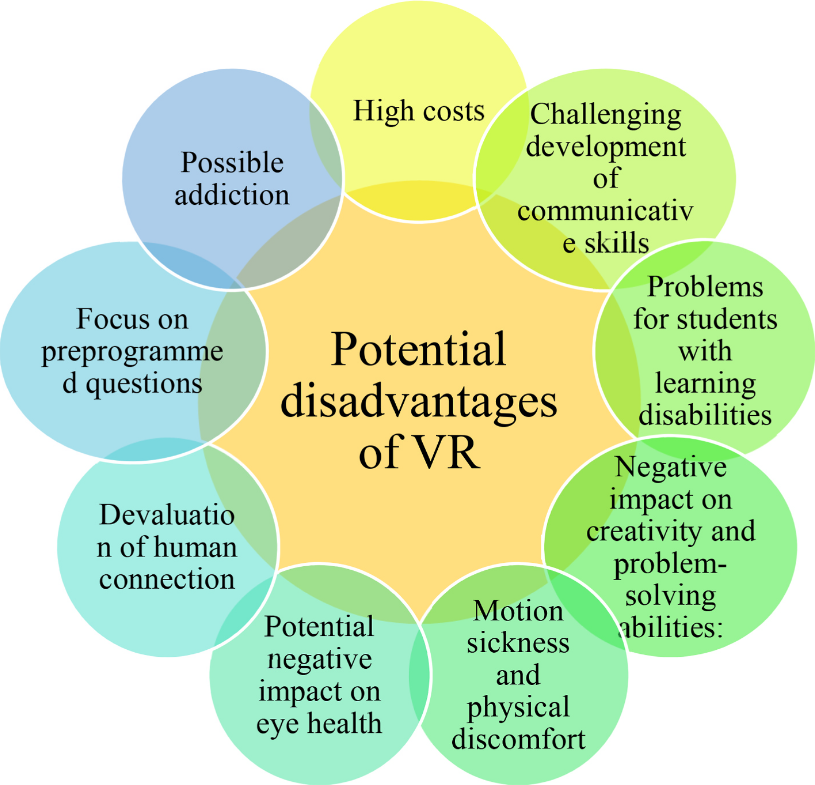
\includegraphics[scale=0.2]{imagenes/exploring-the-effectiveness-of-virtual-reality-in-teaching-maltese-fig-2.png}
   \end{center}
   \caption{Las desventajas de la RV}
   \label{fig:disvr}
   \textit{Nota. }Imagen extraída de \cite{ZAMMIT2023100035}
\end{figure}




\section{Hipotesis}
Las conclusiones que se tienen a llegar de este tema son: 
\begin{enumerate}
   \item La realidad virtual es un nuevo acercamiento a la educación que revolucionara el medio
   \item La realidad virtual ayudara a la retención de conocimiento por medio de las experiencias inmercidas
   \end{enumerate}


\section{Objetivos}

\subsection{Objetivo General}
Demostrar que la realidad virtual puede tener un gran peso en la educación utilizando las herramientas adecuadas, haciendo que las experiencias de aprendizaje sean mas memorables. Se pretende llegar a estas conclusiones por medio de investigaciones previas, y formularios electrónicos repartidos a múltiples grupos sociales, con el motivo de que estas tecnologías se implementen de manera mas cercana al modelo educativo, y, si no se llega al resultado deseado, motivar para que en un futuro se pueda integrar.

\subsection{Objetivos específicos}
\begin{enumerate}
   \item Analizar artículos referentes a la información
   \item Investigar  el impacto de la realidad virtual en la educación
   \item Obtener conclusiones acerca de la información analizada
   \item Escribir un articulo que permita mostrar la información relacionada
   \end{enumerate}


\section{Metodología}
\subsection{Tipo de Estudio}
Para este método se utilizo la cartografía conceptual, método que “sirve para formar y evaluar conceptos esenciales de cada competencia en lo que respecta al saber conocer” \parencite[][p. 16]{tobon2012}. Ademas, se tomo como base la estructura de la metodolgia de \textcite{guzman2020} 
\subsection{Técnica de análisis}
Se utilizaron 8 ejes principales de analisis para clasificar los artículos, denotados anteriormente por \textcite{tobon2012} .
\begin{itemize}
   \item Noción
   \item Categorización
   \item Caracterización
   \item Diferenciación
   \item Clasificación
   \item Vinculación
   \item Metodología
   \item Ejemplificación
\end{itemize}

\begin{table}[!h]
   \caption{Cartografía conceptual}
   \begin{tabular}{p{3.5cm}|p{4.5cm}|p{4.2cm}}
      Eje de análisis & Pregunta Central & Componentes\\
      \hline
      Noción & ¿Cuál es la definición de realidad virtual en el ámbito de la educación, su popularización y en que se destaca? & Definición de términos. Historia. Importancia.\\
      Categorización & ¿A qué clase mayor pertenece el concepto de realidad virtual? & Clase inmediata. Clase que sigue.\\
      Caracterización & ¿Cuáles son las características centrales de la realidad virtual? & Características en base a la noción y la categorización. Explicación de características.\\
      Diferenciación & ¿Cómo se diferencia la realidad virtual de otros conceptos similares? & Definición de los conceptos. Diferencias entre conceptos.\\
      Clasificación & En que rubros se puede clasificar las distintas aplicaciones de la RV & Aplicaciones de la RV en distintas áreas de estudio\\
      Vinculación & Como podemos ligar los beneficios propuestos a dinámicas y cuantificaciones& Muestra de resultados. Resultados a diferencia de otros métodos\\
      Metodología & Que métodos se pueden emplear para probar el funcionamiento de la RV?& Muestra de resultados. Emplearon de la RV a la educación.\\
      Ejemplificación & Como se puede aplicar la RV en el ámbito de la educación? & Casos de aplicación de la RV en una muestra real\\
   \end{tabular}
\end{table}


\subsection{Criterios para la selección de los documentos}

Para esta etapa, se seleccionaron las siguientes partes: palabras clave y bases de datos. Para este trabajo, se eligieron bases de datos que tengan un enfoque científico; en este caso se utilizó Google Académico, Elsevier y SciELO. Los términos de búsqueda implementados fueron “realidad virtual”, “educacion en el aula” y “nuevas tecnologías”.

Cada documento fue seleccionado en base los siguientes criterios:

\begin{enumerate}
   \item Incluir las palabras clave.
   \item Enfocarse en el estudio o análisis del proceso de enseñanza/aprendizaje de la realidad virtual en las aulas.
   \item Tener autor, año y responsable del artículo.
   \item Ser artículos publicados en años recientes.
\end{enumerate}


\subsection{Fases de estudio}

La investigacion se realizo por medio de las siguientes fases:

\begin{itemize}
   \item Fase 1. Se buscaron ls articulos referentes al tema en bases de datos primarias para el tiop de conocimiento, entre ellas Google academico, Elsevier y Scielo.
      \begin{table}[H]
   \caption{Tabla de artículos encontrados, revisados, y utilizados}
   \label{tab:articulos}
      \begin{tabular}{l|l l l}
         \hline
         ~ & Google académico & Elsevier & SciELO\\
         \hline
         Artículos encontrados & 258,000 & 1854 & 30\\
         \hline
         Artículos útiles & 7 & 13 & 2\\
         \hline
      \end{tabular}
\end{table}

   \item Fase 2. Descartar los articulos cuyos criterios no cumplian con los esperados
   \item Fase 3. Realizar la cartografía conceptual
\end{itemize}

%\begin{table}[H]
   \caption{Artículos clasificados en su información}
   \label{tab:articulos-concepto-metod-res-inn}
      \begin{tabular}{|p{3.5cm}|p{3.5cm}|p{3.5cm}|p{3.5cm}|}
         \hline
         Concepto & Metodología & Resultados & innovación\\
         \hline
         \citetitle{rodriguez2021simulacion} & \citetitle{zhan2020augmented} & \citetitle{zamudio2021realidad} & \citetitle{barahona2019cospaces}\\
         \hline
         \citetitle{kaminska2019virtual} & \citetitle{palma2020realidad} & \citetitle{zheng1998virtual} &\\
         \hline
         \citetitle{elmqaddem2019augmented} & \citetitle{jang2021augmented} & \citetitle{chen2020effectiveness} &\\
         \hline
         \citetitle{ZAMMIT2023100035} & \citetitle{marin2022realidad} & \citetitle{OJE2023100033} &\\
         \hline
         \citetitle{YUDINTSEVA2023100018} & \citetitle{GUERRERO2022100002} & \citetitle{LOWELL2023100017} &\\
         \hline
         & \citetitle{RADU2023100011} & &\\
         \hline
         & \citetitle{SHIM2023100010} & &\\
         \hline
         & \citetitle{OYELERE2023100016} & &\\
         \hline
      \end{tabular}
\end{table}

\subsection{Cartografía Conceptual}

\subsubsection{Noción}

“Realidad virtual” proviene de “realidad” (lo real) y “virtual” (lo simulado). Sugiere una representación artificial con potencial realismo. El término se popularizó en la década de 1980, usado inicialmente en informática.La realidad virtual en educación crea entornos de aprendizaje inmersivos que imitan experiencias del mundo real. Destaca la inmersión, interactividad y adaptabilidad a las necesidades del estudiante \parencite{zheng1998virtual}.

La realidad virtual se puede definir como una inmersi{\'o}n humana a un mundo sint{\'e}tico. Esta tecnolog{\'i}a permite a cada usuario mantenerse en un mundo nuevo, en el cual, hay oportunidades inmensas para tanto el aprendizaje, como el entretenimiento\parencite{elmqaddem2019augmented}
\subsubsection{Categorización}

La realidad virtual en la educación se encuentra dentro de la categoría de “tecnología educativa” o “aprendizaje digital”. Las categorías cercanas incluyen “aprendizaje inmersiva” y “simulación educativa”. Su categorías posibles podrían ser “entornos de laboratorio virtual” o “aulas virtuales”. \parencite{barahona2019cospaces, marin2022realidad}

\subsubsection{Caracterización}

La realidad virtual en educación se caracteriza por la inmersión total del estudiante en un entorno virtual interactivo. Esta inmersión implica que los usuarios se sienten completamente inmersos en el entorno virtual, lo que les permite interactuar y aprender de manera efectiva en un contexto simulado. \parencite{zamudio2021realidad}

\input{antecedentes/antecedente-articulo-realidad-virtual-educacion-en-ingles.tex}

\subsubsection{Diferenciación}

Conceptos similares a la realidad virtual en la educación incluyen la “realidad aumentada” y el “aprendizaje en línea”. La “realidad aumentada” superpone elementos virtuales en el mundo real, mientras que el “aprendizaje en línea” implica la enseñanza y el aprendizaje a través de Internet. La realidad virtual sumerge a los usuarios en entornos virtuales completamente simulados, mientras que la realidad aumentada añade elementos virtuales al mundo real. El aprendizaje en línea se refiere a la educación basada en la web sin necesidad de inmersión en entornos virtuales \parencite{garcia2020, LOWELL2023100017}

Los resultados entre una educacion hecha por un sistema tradicional a comparaci{\'o}n de uno utilizando la realidad virtual llegan a mostrar distintos resultados, los cuales arrojan resultados completamente distintos, en unos, se denota una mejo experiencia de aprendizaje, mientras que en otras, la mejora no es significativa. \parencite{palma2020realidad, SHIM2023100010, GUERRERO2022100002}

\subsubsection{Clasificación}

La RV ha sido un medio en el cual múltiples áreas del estudio han sido adaptadas por esta, como lo puede ser en la medicina, donde ha habido casos de entrenamiento para enfermeros/as para determinar pacientes en potencia de tener COVID-19 \parencite{GUERRERO2022100002}. A esto, no solo se excluye a este tipo de temas, sino que se puede aplicar tambi{\'e}n a la educaci{\'o}n b{\'a}sica \parencite{marin2022realidad}.

\subsubsection{Vinculación}

Se notaron en los resultados de \textcite{SHIM2023100010} que la RV si puede crear una diferencia a la hora del aprendizaje, mas no es abismal, y no trata todos los aspectos de la educación moral. Al igual, en estudios hacia enfermeras se notaron mucho mas competentes aquellas con simulaciones, que, al ser evaluadas antes y después de tomar una simulación de alta fidelidad, hubo un gran incremento en los promedios de al menos 20.67 puntos sobre 100. \parencite{GUERRERO2022100002}

\subsubsection{Metodología}
Utilizando métodos introductorios a la realidad virtual, como lo puede ser la realidad aumentada, se pueden tomar pruebas que incluyan rubros como la física, y hacer sesiones de tutoría remotas. Con ello, se pueden visualizar conceptos digitales a nuestra realidad con los que la experiencia de aprendizaje es mas agradable, y múltiples conceptos se pueden materializar en imágenes a tiempo real \parencite{RADU2023100011}

\subsubsection{Ejemplificación}

Un ejemplo aplicado de la RV en la educación son los estudios y experimentos hechos por \textcite{SHIM2023100010}, donde se aplica hacia un grupo de niños donde el rumbo de la investigación es hacia la educación moral, componente importante para el desarrollo del ser humano, y que, se demostró que la sensibilidad moral mostró un incremento significativo, mas no el juicio moral. Y en otros estudios, \textcite{OJE2023100033} muestra la educaci{\'o}n asistida con RV, y con ello, que en un futuro se puedan desarrollar m{\'a}s contenidos hacia la educaci{\'o}n en ingenier{\'i}a en realidad virtual.

En tiempos actuales, se ha notado como la realidad virtual ha empezado a formar parte de muchas áreas del trabajo y de la vida, como lo pueden ser la medicina, entretenimiento, educación, etc. Numerosos estudios han utilizado la realidad virtual en la educación, y han desarrollado aplicaciones, por ejemplo, donde se apoya a los estudiantes a entender conceptos de la computación como lo puede ser un \textit{bubble sort}. \parencite{OYELERE2023100016} 



\section{Resultados}

Después del análisis de las fuentes de información, la RV es una tecnología que podría ayudar a mejorar el sistema de educación actual, ya que en este hay numerosas ventajas y desventajas al implementarlo en un modelo educativo.
%\begin{table}[H]
%   \caption{Uso de RV respecto a cada fuente de información}
%   \label{tab:validacionrv}
%   \begin{center}
%      \begin{tabular}{p{3cm}|p{10cm}}
%         \hline
%         Fuente & Conclusión\\
%         \hline
%         \citetitle{ZAMMIT2023100035} & Utilizar la RV como una herramienta, mas no utilizarla totalmente\\
%         \citetitle{GUERRERO2022100002} & Implementar la RV como un nuevo sistema\\
%         \citetitle{SHIM2023100010} & La RV puede funcionar para conocimientos y habilidades especificas, pero no todas\\
%         \hline
%      \end{tabular}
%   \end{center}
%\end{table}
En base a los resultados, es clara la visión en que la RV podría llegar a mejorar la educación, sin embargo, esta no es viable reemplazarla totalmente, ya que puede haber casos donde la sobre estimulación puede llegar a deslindar desde la ruta hecha para el aprendizaje. Para esta hay que mantener una moderacion, ya que puede llegar a ser perjudicial el solo trabajar con RV en distintas areas. Asi como es beneficioso, tiene desventajas que pueden llegar a ser decisivas.


\printbibliography
\end{document}



\printbibliography
\end{document}
